\chapter{GİRİŞ}



Basit iki terimle \acrfull{lbp} ve \acrfull{svm} kısaltmaları anlatabiliriz. İster kısaltmasını \acrshort{svm}, isterseniz de uzun açılımını \acrlong{svm} yazdırabilirsiniz. Bunu yapabilmek için dosyanın başında terimleri tanımlamanız gereklidir. İsterseniz matematik terimlerini de, örneğin \acrshort{pca} böyle tanımlayabilirsiniz. Uzun uzun \acrfull{pca} yazmanız gerekmez. 
\acrfull{svm}
\acrshort{lbp}
\lipsum[16-20]
68 farklı noktanın konumları Şekil-\ref{fig:68point}'de gösterilmiştir.
\lipsum[3]
Öznitelik seçimi için boyut indirgeme aracı olan \acrfull{pca} , \acrfull{sffs} ve \acrfull{sbfs} uygulanmıştır.  
\begin{figure}[ht]
\centering
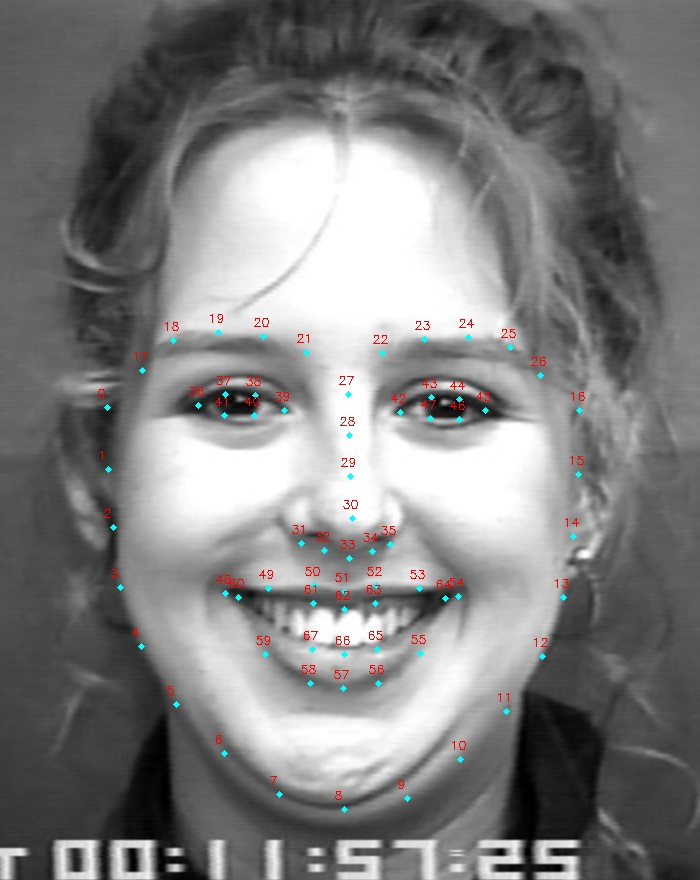
\includegraphics[trim={2cm 1.5cm 2cm 8cm},clip,width=0.75\textwidth]{gorseller/68point.jpg}
\caption{Nirengi Noktaları}\label{fig:68point}
\end{figure}
%[trim={5cm 0 0 0},clip] <left> <lover> <right> <upper>

\lipsum[5-8]

% Teorem yazmak isterseniz:
% \begin{theorem}[Öklid]
%  İki noktadan bir ve yalnız bir doğru geçer.
% \end{theorem}

% İspat yazmak isterseniz:
% \begin{ispat}[Tezin en önemli ispatı]
% x=10
% \end{ispat}
% \lipsum[1-2]
% \begin{figure}[h]
% \centering
% 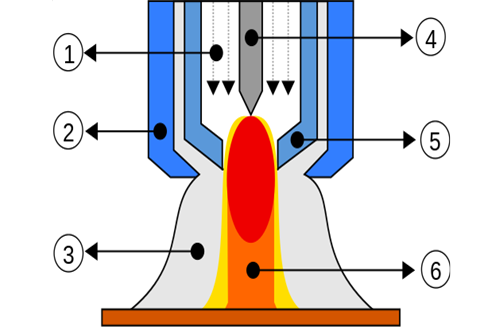
\includegraphics[width=\textwidth]{gorseller/ptaTorc}
% \caption{PTA Torç}\label{fig:PtaTorc1}
% \end{figure}
% \lipsum[1-2]
% \begin{table}
% \centering
% \caption{Deneme Tablosu.}\label{tab:den1}
% \begin{tabular}{|l|l|l|}
% \hline
% sıra   & sayı   & toplam \\ \hline
% 1      & 2      & 3      \\ \hline
% Kelime & deneme & son    \\ \hline
% \end{tabular}
% \end{table}


% %\section{Giriş Birinci Derece Başlık}
% \lipsum[1-2]
% \begin{figure}[h]
% \centering
% 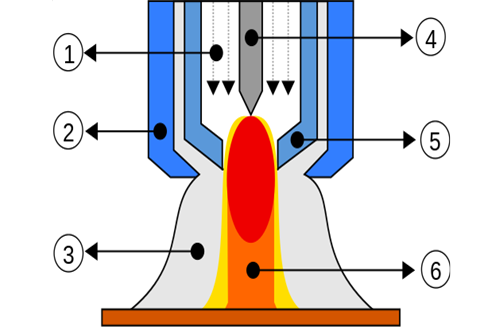
\includegraphics[width=\textwidth]{gorseller/ptaTorc}
% \caption{PTA Torç}\label{fig:PtaTorc1}
% \end{figure}
% \lipsum[1-2]
% \begin{table}
% \centering
% \caption{Deneme Tablosu.}\label{tab:den1}
% \begin{tabular}{|l|l|l|}
% \hline
% sıra   & sayı   & toplam \\ \hline
% 1      & 2      & 3      \\ \hline
% Kelime & deneme & son    \\ \hline
% \end{tabular}
% \end{table}
% Teorem yazmak isterseniz:
% \begin{theorem}[Öklid]
%  İki noktadan bir ve yalnız bir doğru geçer.
% \end{theorem}

% İspat yazmak isterseniz:
% \begin{ispat}[Tezin en önemli ispatı]
% x=10
% \end{ispat}

% %\subsection{Giriş ikinci derece başlık}
% \lipsum[1-2]
% \begin{figure}[h]
% \centering
% 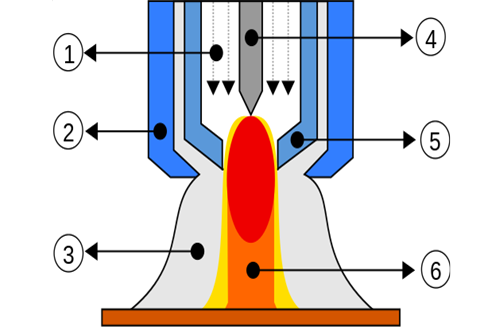
\includegraphics[width=\textwidth]{gorseller/ptaTorc}
% \caption{PTA Torç}\label{fig:PtaTorc1}
% \end{figure}
% \lipsum[1-2]
% \begin{table}
% \centering
% \caption{Deneme Tablosu.}\label{tab:den1}
% \begin{tabular}{|l|l|l|}
% \hline
% sıra   & sayı   & toplam \\ \hline
% 1      & 2      & 3      \\ \hline
% Kelime & deneme & son    \\ \hline
% \end{tabular}
% \end{table}

% Teorem yazmak isterseniz:
% \begin{theorem}[Öklid]
%  İki noktadan bir ve yalnız bir doğru geçer.
% \end{theorem}

% İspat yazmak isterseniz:
% \begin{ispat}[Tezin en önemli ispatı]
% x=10
% \end{ispat}

% %\subsubsection{Giriş dördüncü derece başlık}
% \lipsum[1-2]
% \begin{figure}[h]
% \centering
% 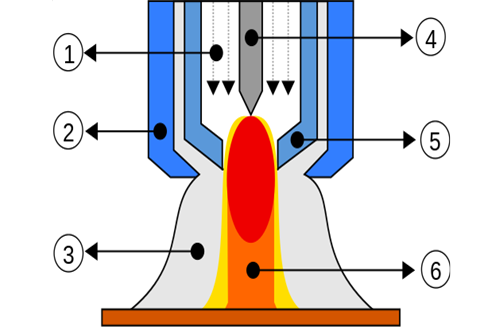
\includegraphics[width=\textwidth]{gorseller/ptaTorc}
% \caption{PTA Torç}\label{fig:PtaTorc1}
% \end{figure}
% \lipsum[1-2]
% \begin{table}
% \centering
% \caption{Deneme Tablosu.}\label{tab:den1}
% \begin{tabular}{|l|l|l|}
% \hline
% sıra   & sayı   & toplam \\ \hline
% 1      & 2      & 3      \\ \hline
% Kelime & deneme & son    \\ \hline
% \end{tabular}
% \end{table}

% Teorem yazmak isterseniz:
% \begin{theorem}[Öklid]
%  İki noktadan bir ve yalnız bir doğru geçer.
% \end{theorem}

% İspat yazmak isterseniz:
% \begin{ispat}[Tezin en önemli ispatı]
% x=10
% \end{ispat}